%% LaTeX2e class for student theses
%% sections/appendix.tex
%%
%% Karlsruhe Institute of Technology
%% Institute for Program Structures and Data Organization
%% Chair for Software Design and Quality (SDQ)
%%
%% Dr.-Ing. Erik Burger
%% burger@kit.edu
%%
%% Version 1.3.5, 2020-06-26

\iflanguage{english}
{\chapter{Appendix}}    % english style
{\chapter{Anhang}}      % German style
\label{chap:appendix}


%% -------------------
%% | Example content |
%% -------------------
\section{Resultate Experiment 2}
\label{sec:appendix:exp2}
\begin{figure} [ht]
  \centering
  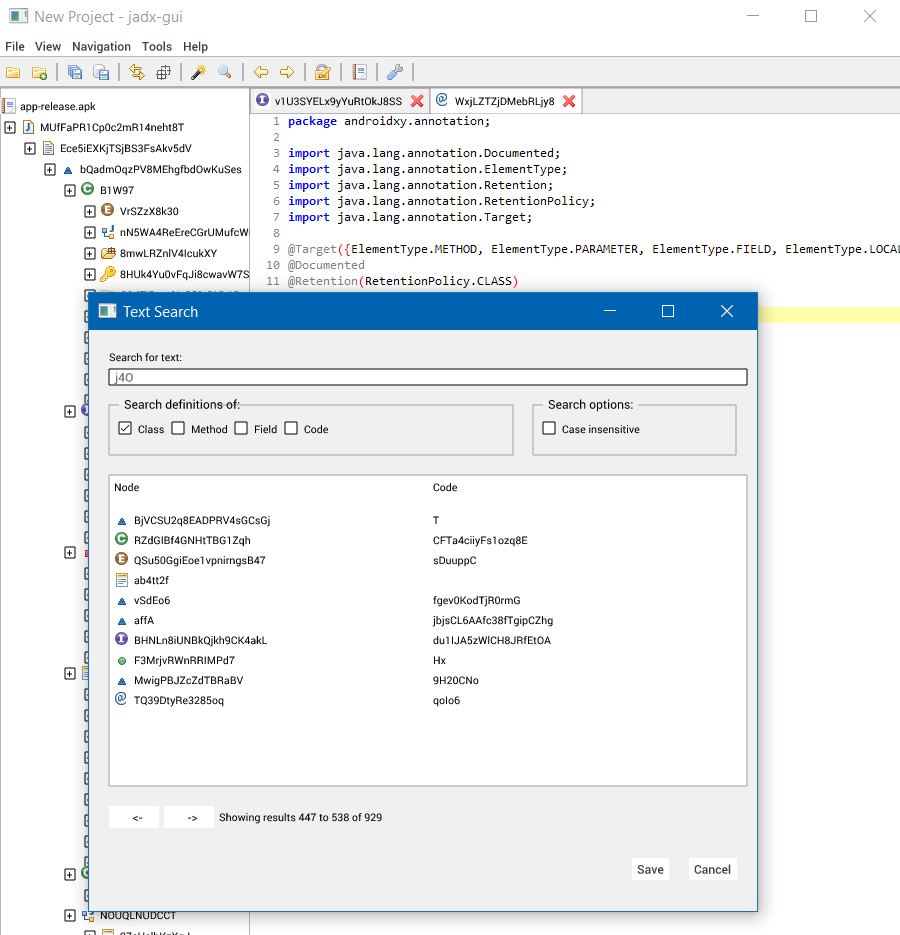
\includegraphics[height=0.67\textheight]{bilder/result_exp2/0.png}
  % 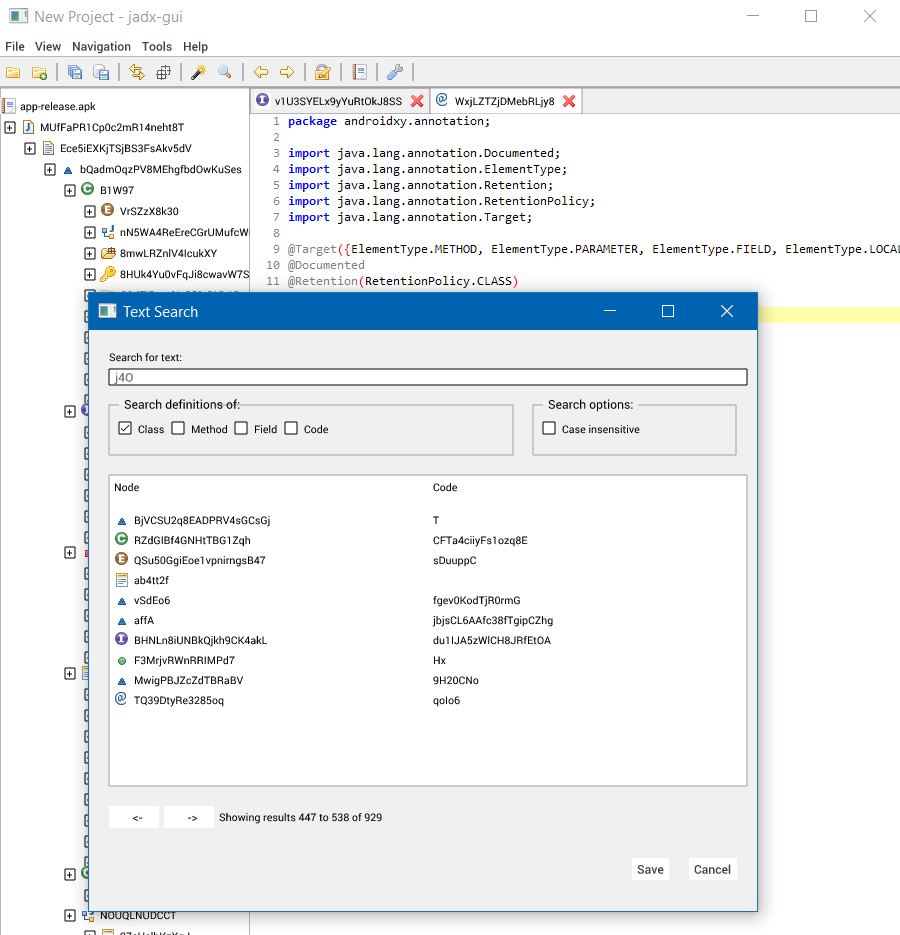
\includegraphics[width=\textwidth]{bilder/result_exp2/0.png}

  \caption{Experiment 2: Originalbild 1 aus Abb.~\ref{exp2_image:1} in hoher Auflösung}
\end{figure}

\begin{figure} [ht]
  \centering
  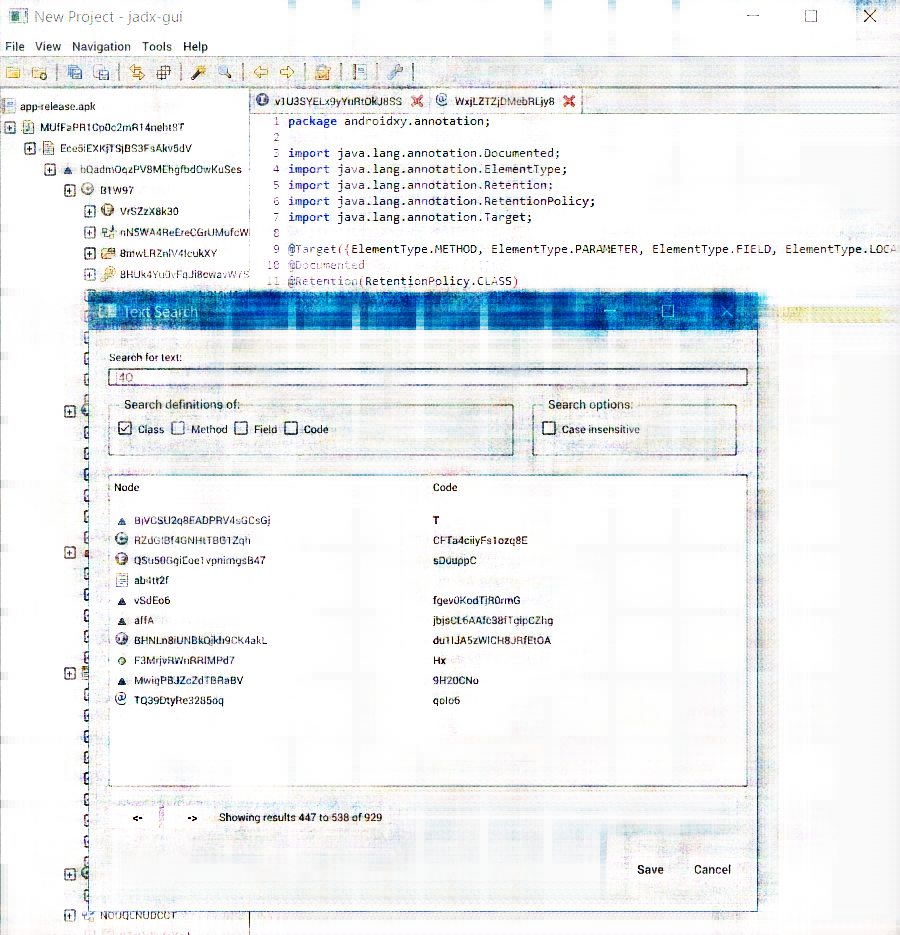
\includegraphics[width=\textwidth]{bilder/result_exp2/0_pred_a1.png}

  \caption{Experiment 2: Ausgabe des Autoencoders~\ref{a1} zu Bild 1 aus Abb.~\ref{exp2_image:1} in hoher Auflösung}
\end{figure}

\begin{figure} [ht]
  \centering
  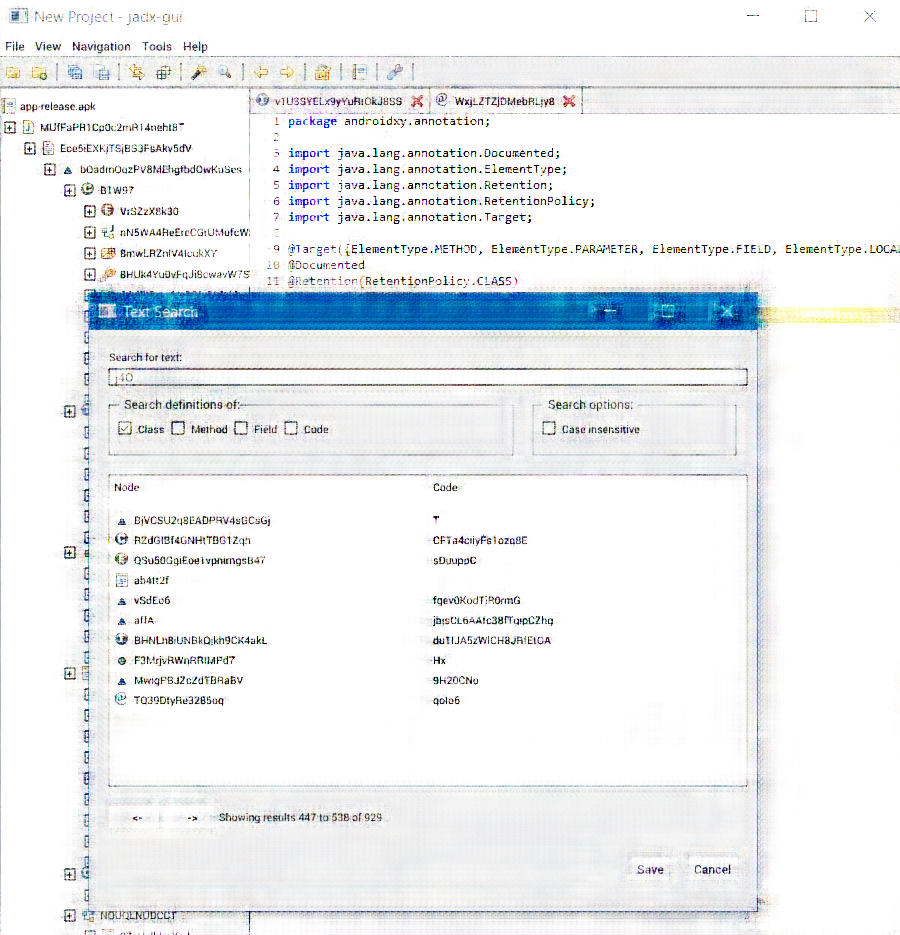
\includegraphics[width=\textwidth]{bilder/result_exp2/0_pred_a2.png}

  \caption{Experiment 2: Ausgabe des Autoencoders~\ref{a2} zu Bild 1 aus Abb.~\ref{exp2_image:1} in hoher Auflösung}
\end{figure}

\begin{figure} [ht]
  \centering
  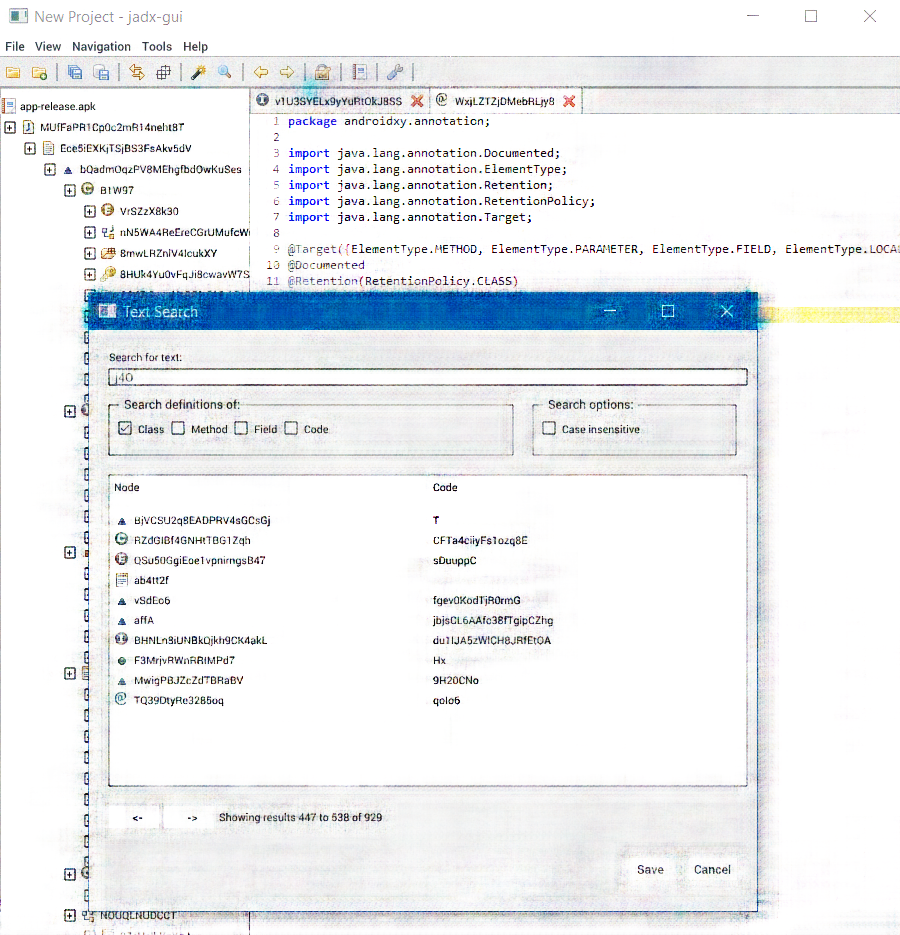
\includegraphics[width=\textwidth]{bilder/result_exp2/0_pred_a3.png}

  \caption{Experiment 2: Ausgabe des Autoencoders~\ref{a3} zu Bild 1 aus Abb.~\ref{exp2_image:1} in hoher Auflösung}
\end{figure}

\begin{figure} [ht]
  \centering
  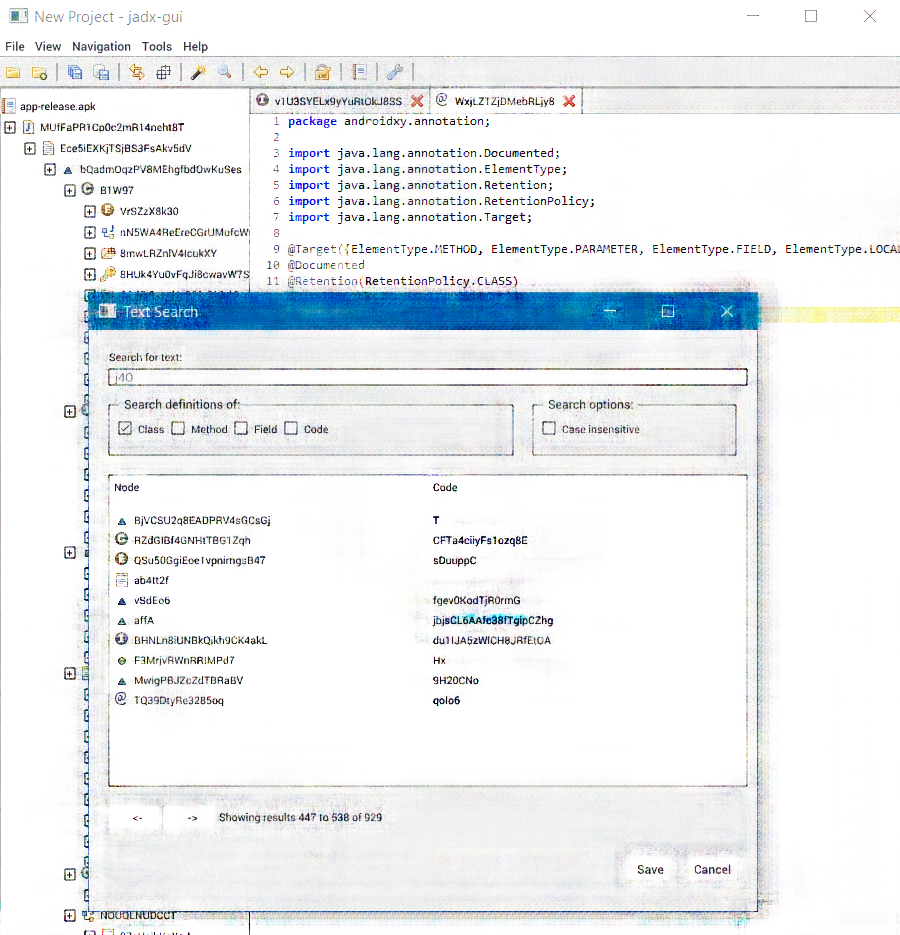
\includegraphics[width=\textwidth]{bilder/result_exp2/0_pred_a4.png}

  \caption{Experiment 2: Ausgabe des Autoencoders~\ref{a4} zu Bild 1 aus Abb.~\ref{exp2_image:1} in hoher Auflösung}
\end{figure}

\label{sec:appendix:exp2_2}
\begin{figure} [ht]
  \centering
  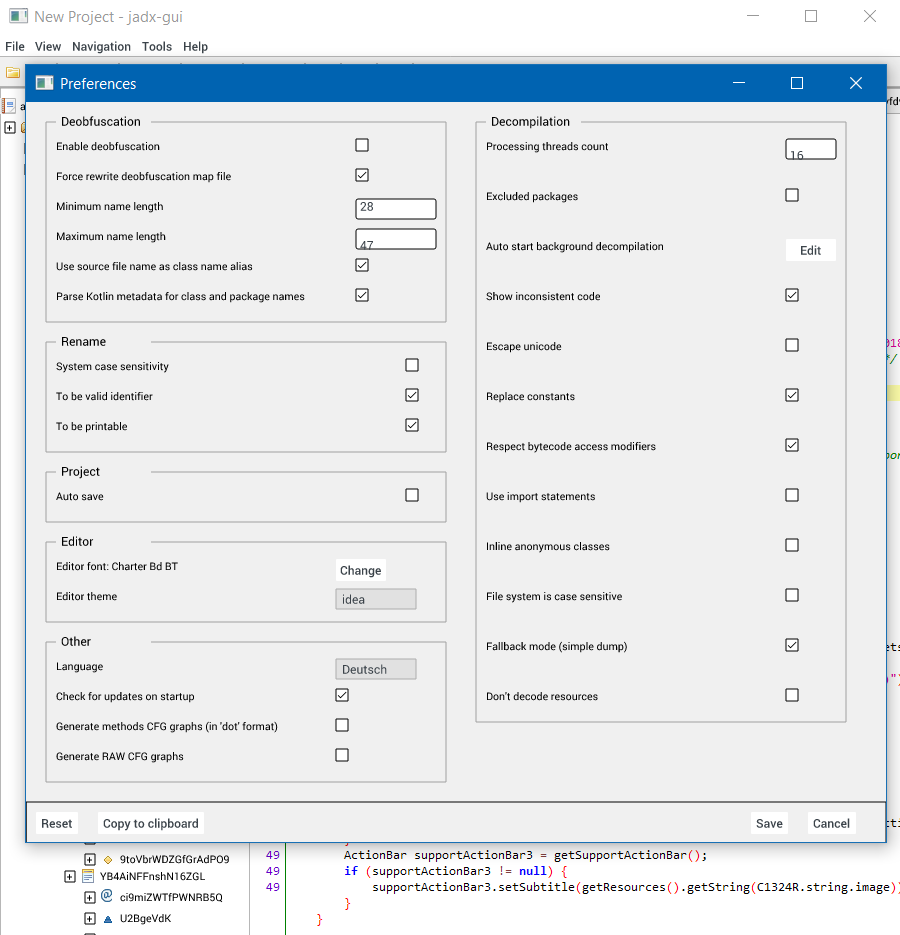
\includegraphics[width=\textwidth]{bilder/result_exp2/1.png}

  \caption{Experiment 2: Originalbild 2 aus Abb.~\ref{exp2_image:2} in hoher Auflösung}
\end{figure}

\begin{figure} [ht]
  \centering
  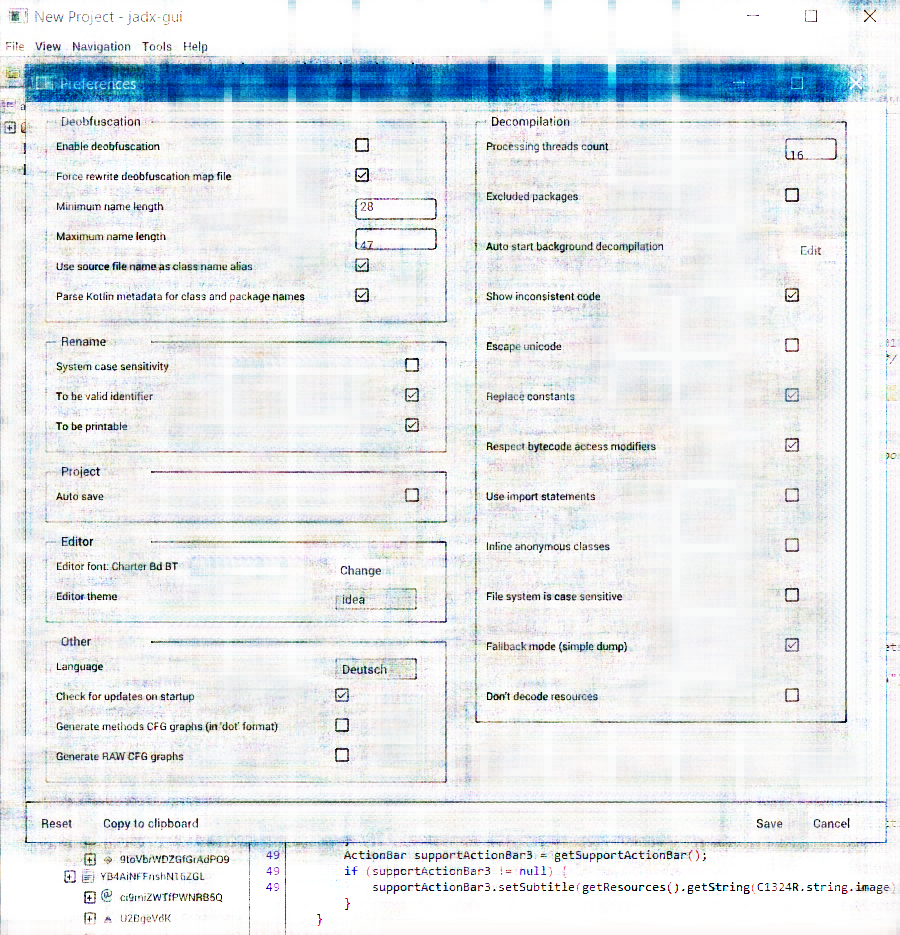
\includegraphics[width=\textwidth]{bilder/result_exp2/1_pred_a1.png}

  \caption{Experiment 2: Ausgabe des Autoencoders~\ref{a1} zu Bild 2 aus Abb.~\ref{exp2_image:2} in hoher Auflösung}
\end{figure}

\begin{figure} [ht]
  \centering
  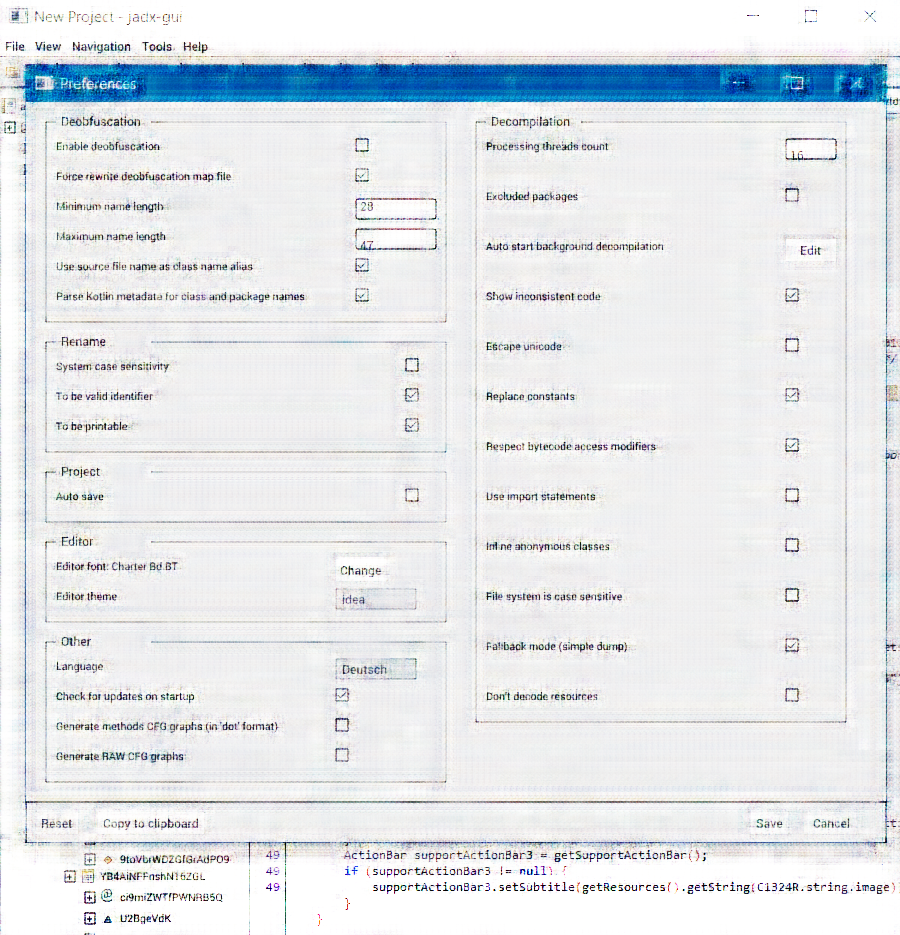
\includegraphics[width=\textwidth]{bilder/result_exp2/1_pred_a2.png}

  \caption{Experiment 2: Ausgabe des Autoencoders~\ref{a2} zu Bild 2 aus Abb.~\ref{exp2_image:2} in hoher Auflösung}
\end{figure}

\begin{figure} [ht]
  \centering
  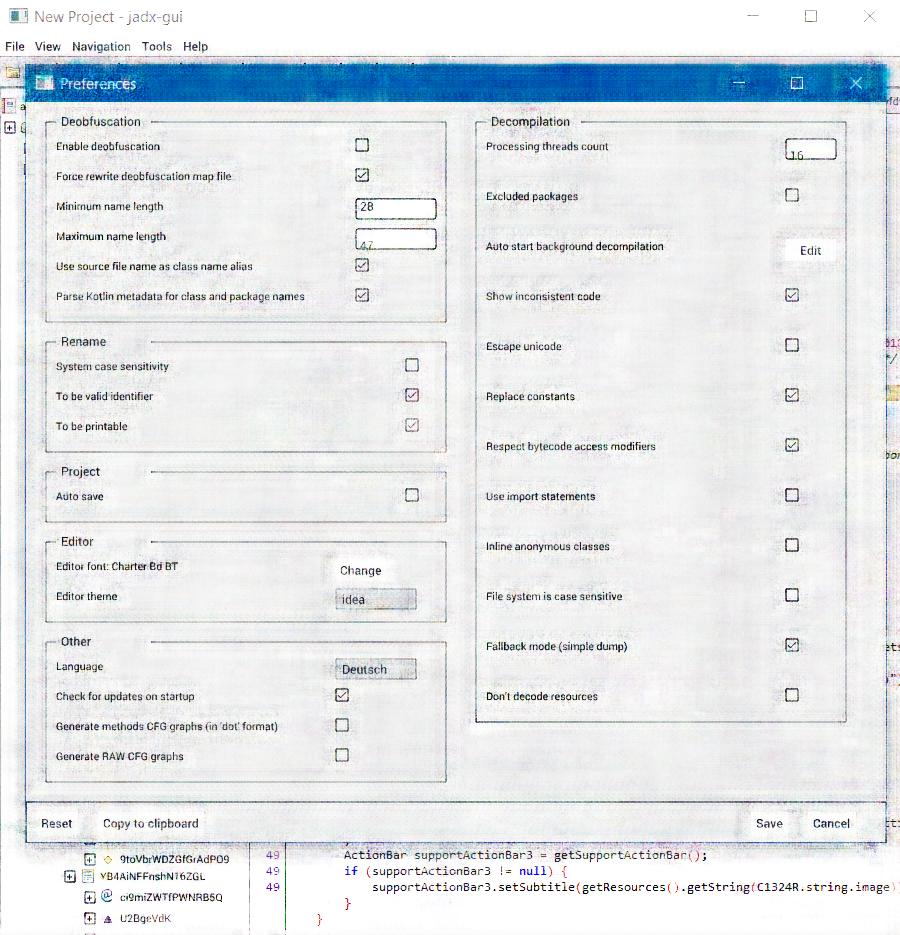
\includegraphics[width=\textwidth]{bilder/result_exp2/1_pred_a3.png}

  \caption{Experiment 2: Ausgabe des Autoencoders~\ref{a3} zu Bild 2 aus Abb.~\ref{exp2_image:2} in hoher Auflösung}
\end{figure}

\begin{figure} [ht]
  \centering
  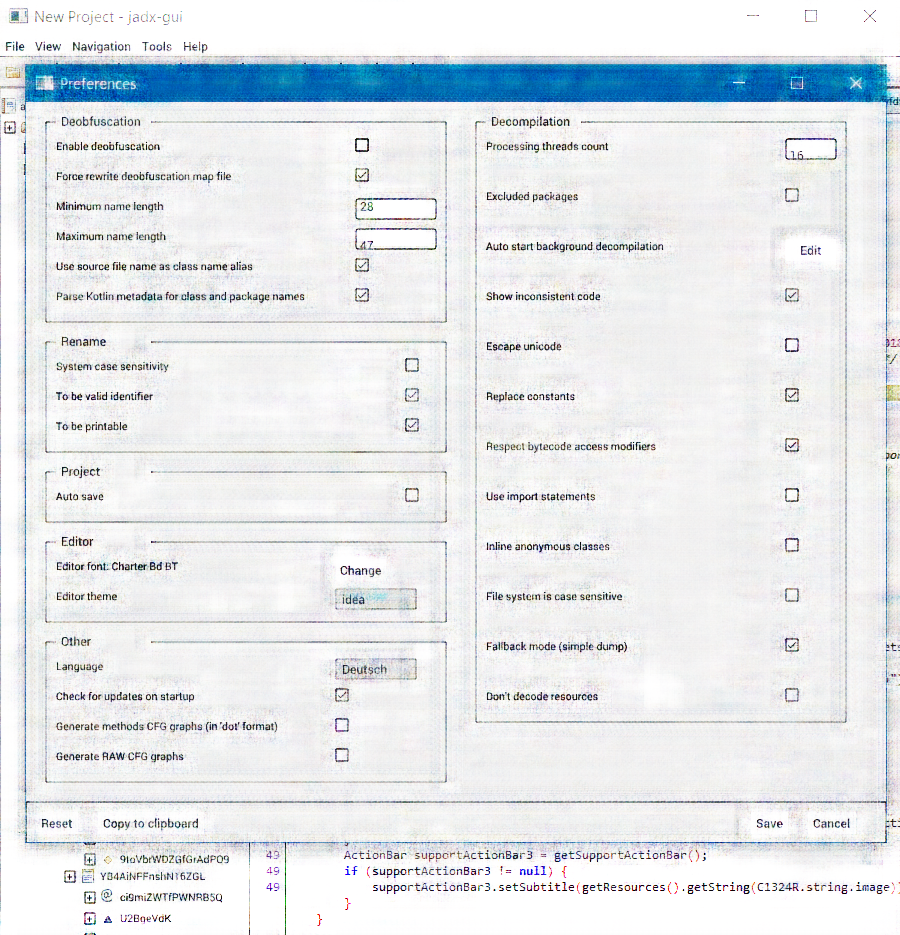
\includegraphics[width=\textwidth]{bilder/result_exp2/1_pred_a4.png}

  \caption{Experiment 2: Ausgabe des Autoencoders~\ref{a4} zu Bild 2 aus Abb.~\ref{exp2_image:2} in hoher Auflösung}
\end{figure}

\section{Resultate Experiment 3}
\label{sec:appendix:exp3}

\begin{figure} [ht]
  \centering
  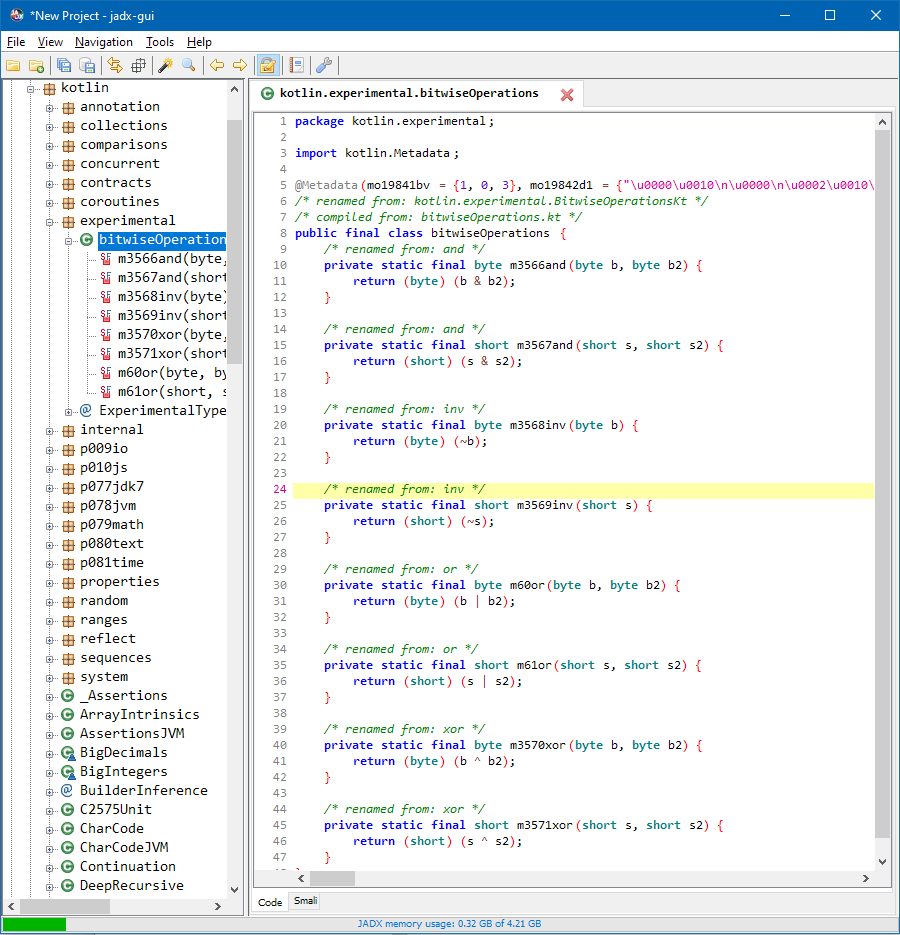
\includegraphics[width=\textwidth]{bilder/result_exp3/1.png}
  % 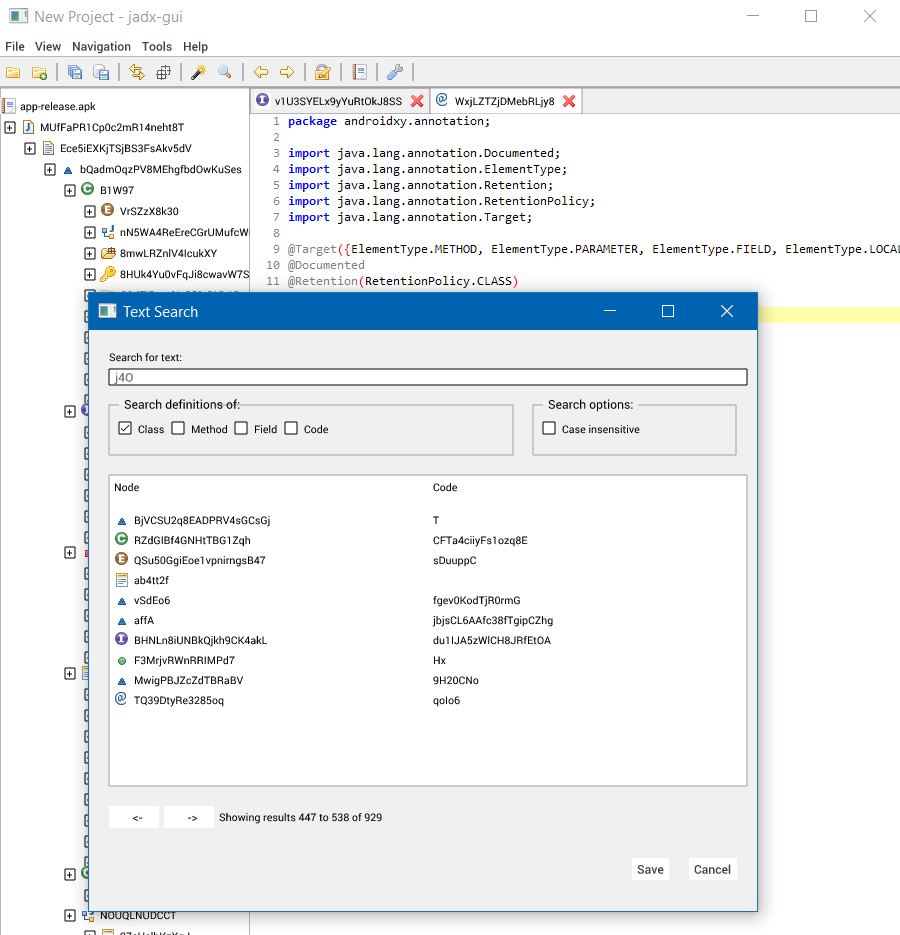
\includegraphics[width=\textwidth]{bilder/result_exp2/0.png}

  \caption{Experiment 3: Originalbild 1 aus Abb.~\ref{exp3_image:1} in hoher Auflösung}
\end{figure}

\begin{figure} [ht]
  \centering
  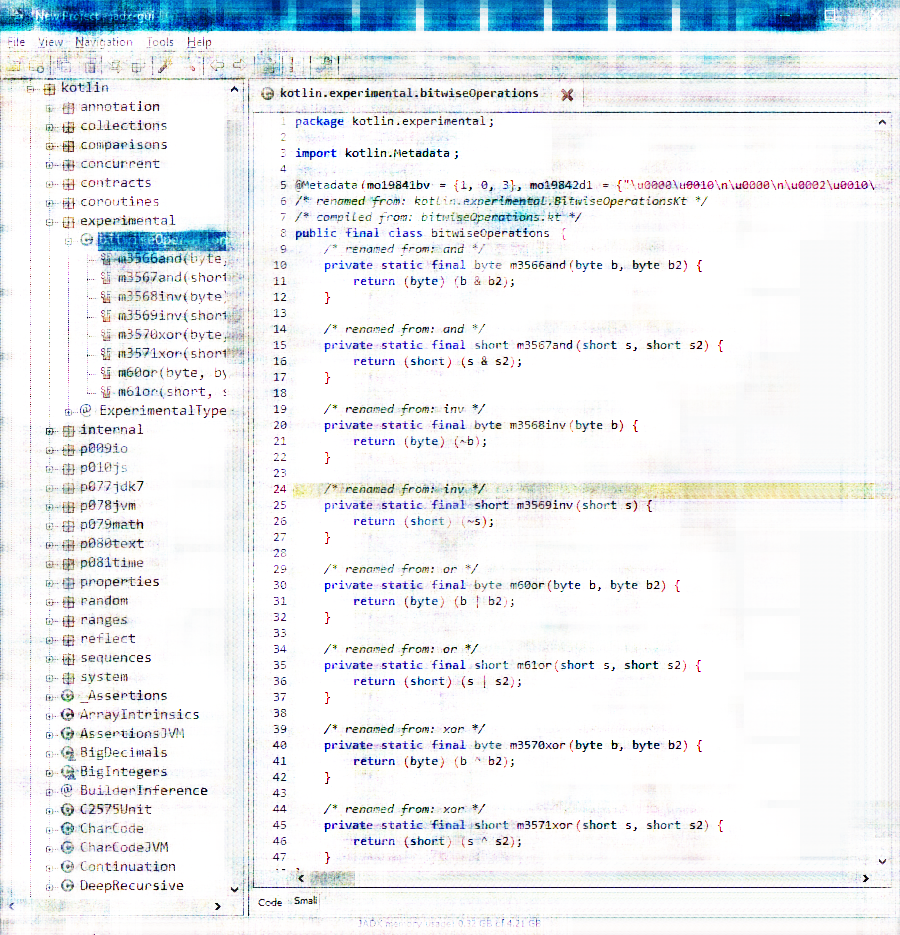
\includegraphics[width=\textwidth]{bilder/result_exp3/1_pred_a1.png}

  \caption{Experiment 3: Ausgabe des Autoencoders~\ref{a1} zu Bild 1 aus Abb.~\ref{exp3_image:1} in hoher Auflösung}
\end{figure}

\begin{figure} [ht]
  \centering
  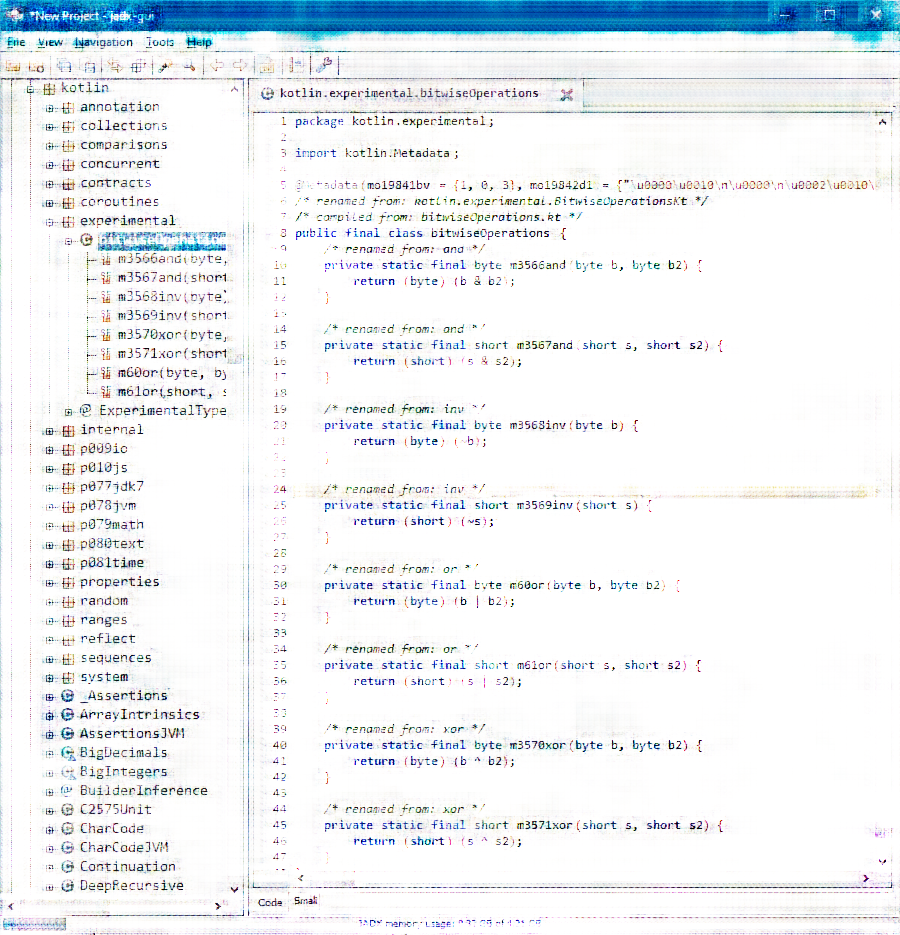
\includegraphics[width=\textwidth]{bilder/result_exp3/1_pred_a2.png}

  \caption{Experiment 3: Ausgabe des Autoencoders~\ref{a2} zu Bild 1 aus Abb.~\ref{exp3_image:1} in hoher Auflösung}
\end{figure}

\begin{figure} [ht]
  \centering
  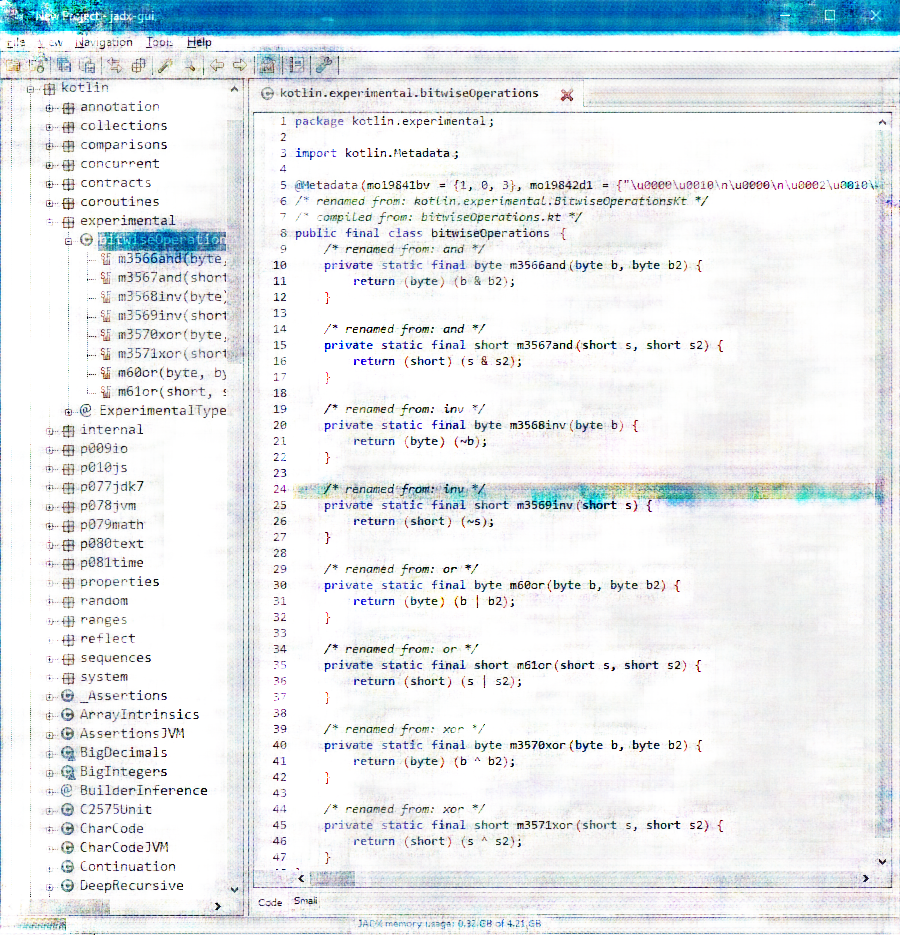
\includegraphics[width=\textwidth]{bilder/result_exp3/1_pred_a3.png}

  \caption{Experiment 3: Ausgabe des Autoencoders~\ref{a3} zu Bild 1 aus Abb.~\ref{exp3_image:1} in hoher Auflösung}
\end{figure}

\begin{figure} [ht]
  \centering
  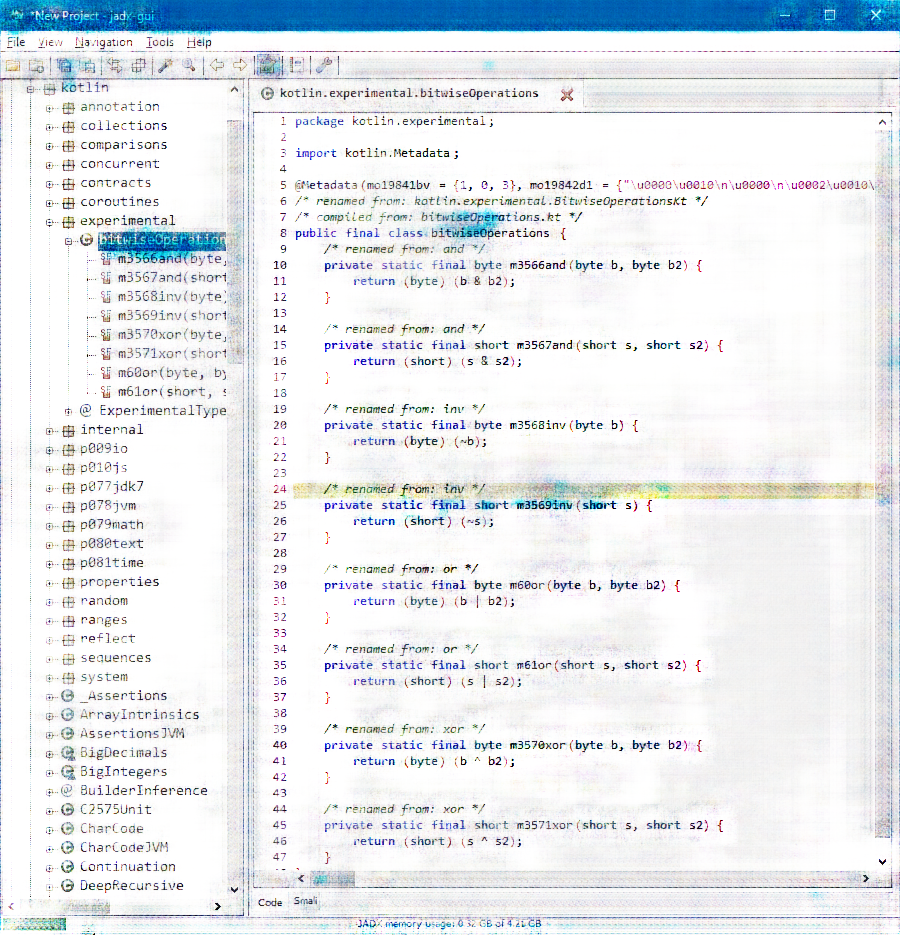
\includegraphics[width=\textwidth]{bilder/result_exp3/1_pred_a4.png}

  \caption{Experiment 3: Ausgabe des Autoencoders~\ref{a4} zu Bild 1 aus Abb.~\ref{exp3_image:1} in hoher Auflösung}
\end{figure}

\label{sec:appendix:exp3_2}
\begin{figure} [ht]
  \centering
  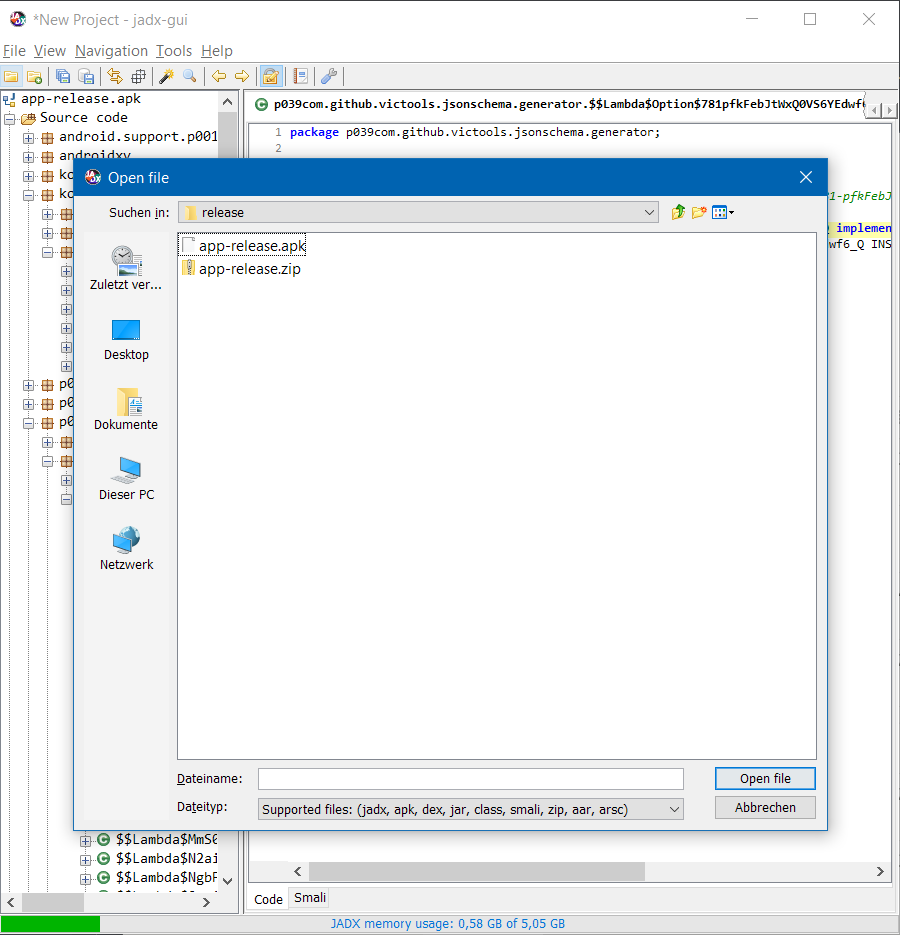
\includegraphics[width=\textwidth]{bilder/result_exp3/2.png}

  \caption{Experiment 3: Originalbild 2 aus Abb.~\ref{exp3_image:2} in hoher Auflösung}
\end{figure}

\begin{figure} [ht]
  \centering
  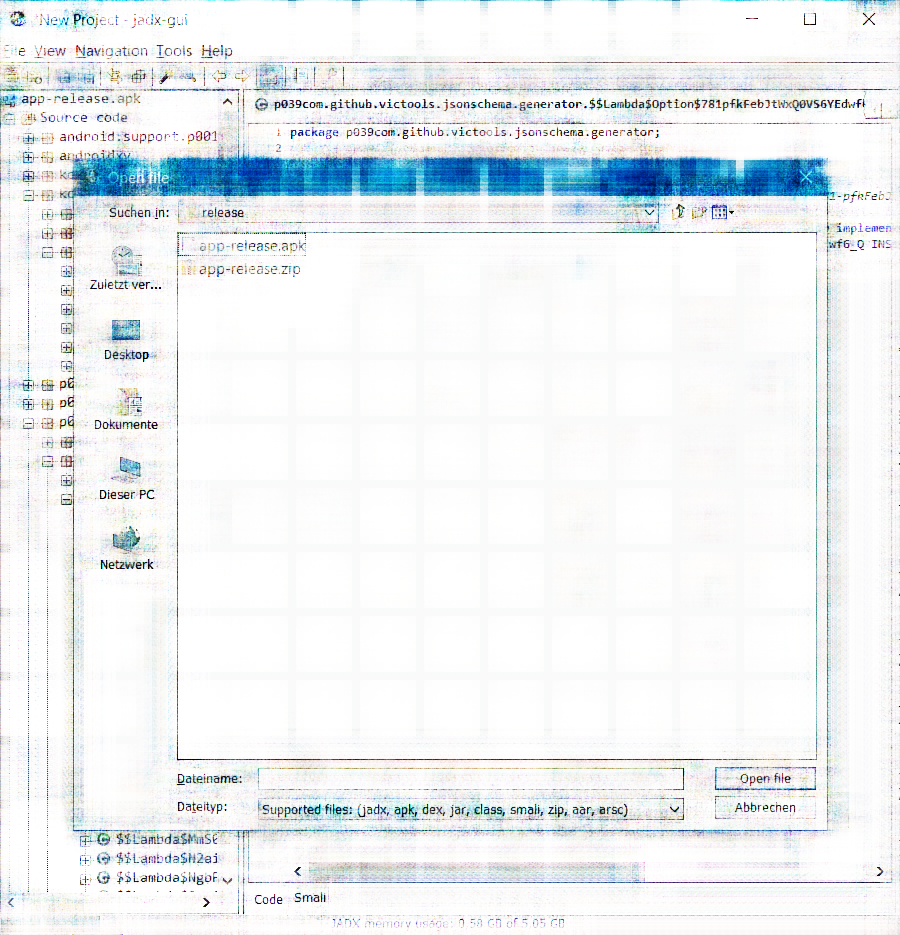
\includegraphics[width=\textwidth]{bilder/result_exp3/2_pred_a1.png}

  \caption{Experiment 3: Ausgabe des Autoencoders~\ref{a1} zu Bild 2 aus Abb.~\ref{exp3_image:2} in hoher Auflösung}
\end{figure}

\begin{figure} [ht]
  \centering
  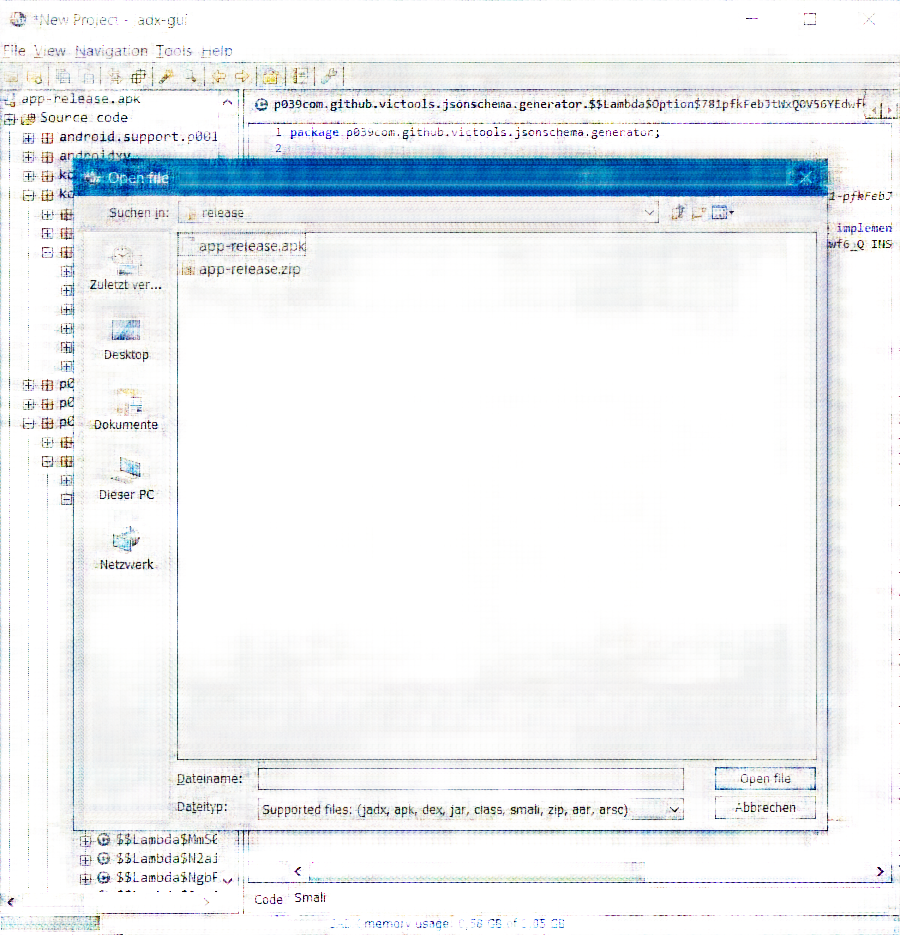
\includegraphics[width=\textwidth]{bilder/result_exp3/2_pred_a2.png}

  \caption{Experiment 3: Ausgabe des Autoencoders~\ref{a2} zu Bild 2 aus Abb.~\ref{exp3_image:2} in hoher Auflösung}
\end{figure}

\begin{figure} [ht]
  \centering
  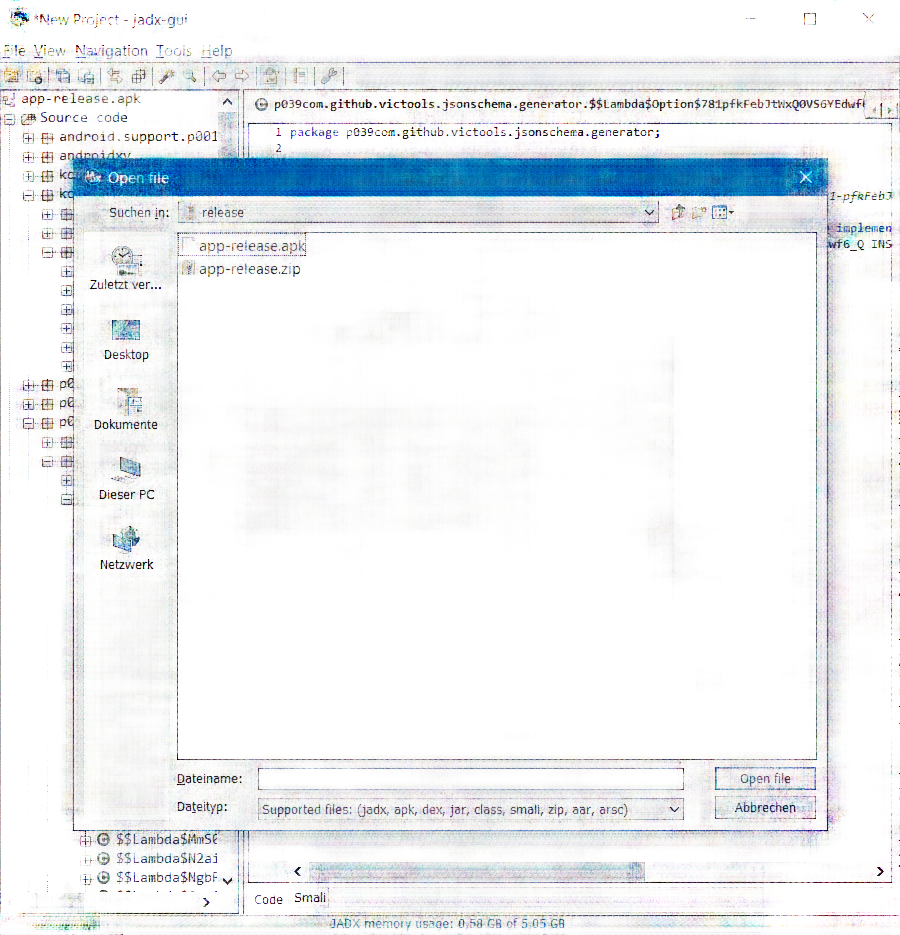
\includegraphics[width=\textwidth]{bilder/result_exp3/2_pred_a3.png}

  \caption{Experiment 3: Ausgabe des Autoencoders~\ref{a3} zu Bild 2 aus Abb.~\ref{exp3_image:2} in hoher Auflösung}
\end{figure}

\begin{figure} [ht]
  \centering
  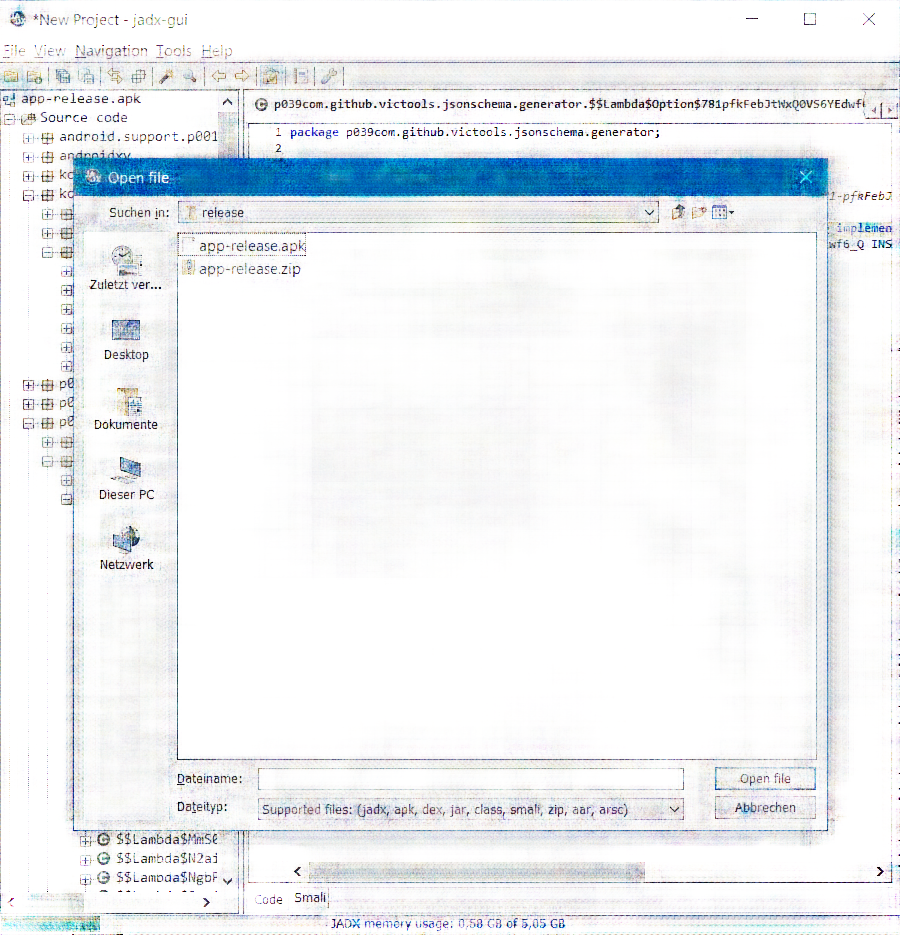
\includegraphics[width=\textwidth]{bilder/result_exp3/2_pred_a4.png}

  \caption{Experiment 3: Ausgabe des Autoencoders~\ref{a4} zu Bild 2 aus Abb.~\ref{exp3_image:2} in hoher Auflösung}
\end{figure}


\section{Resultate Experiment 4}
\label{sec:appendix:exp4}

\begin{figure} [ht]
  \centering
  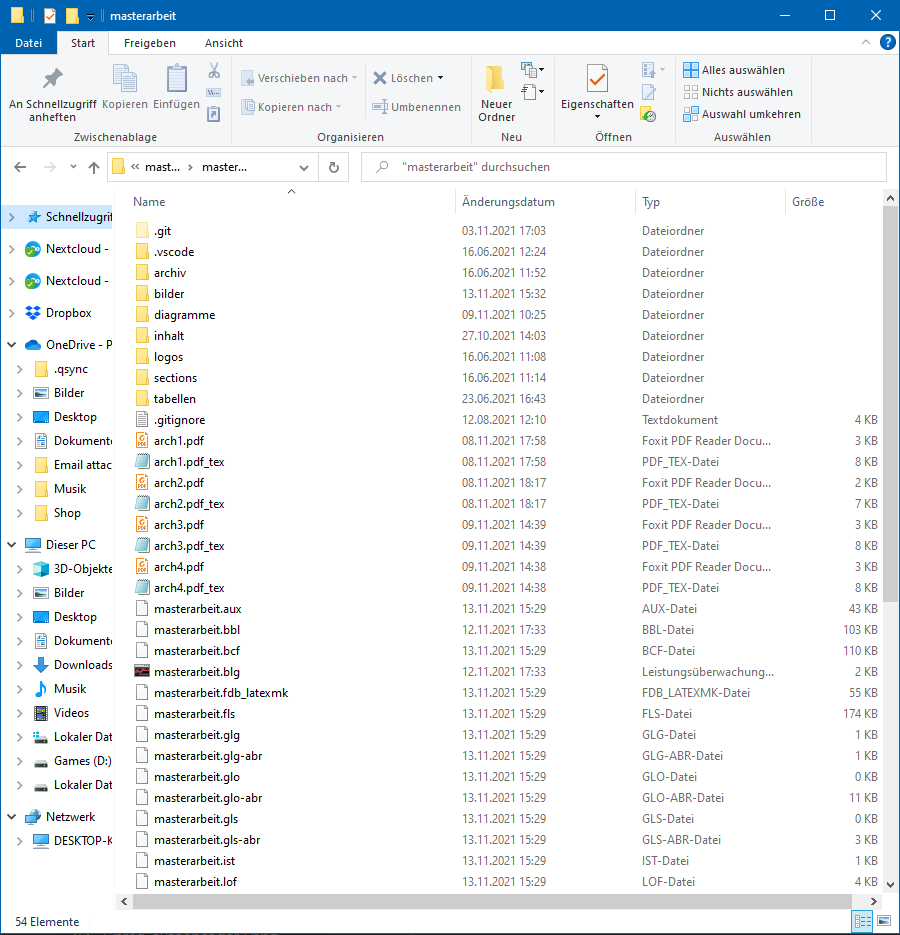
\includegraphics[width=\textwidth]{bilder/result_exp4/3.png}
  % 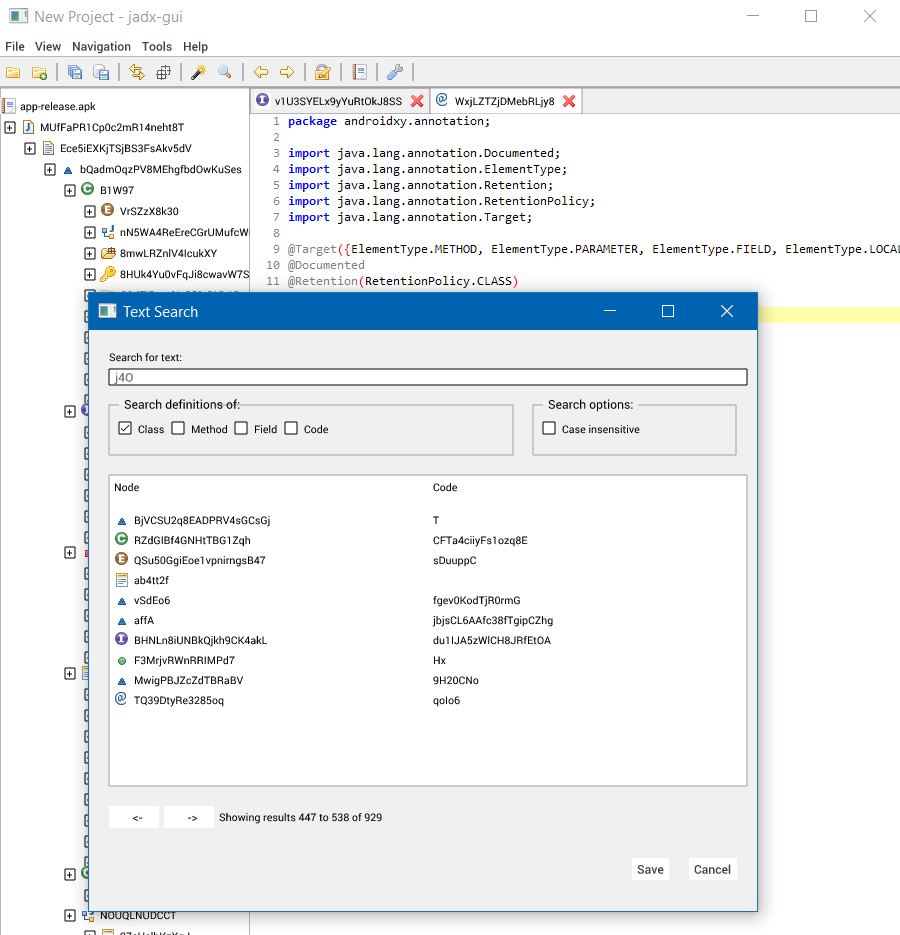
\includegraphics[width=\textwidth]{bilder/result_exp2/0.png}

  \caption{Experiment 4: Originalbild 1 aus Abb.~\ref{exp4_image:1} in hoher Auflösung}
\end{figure}

\begin{figure} [ht]
  \centering
  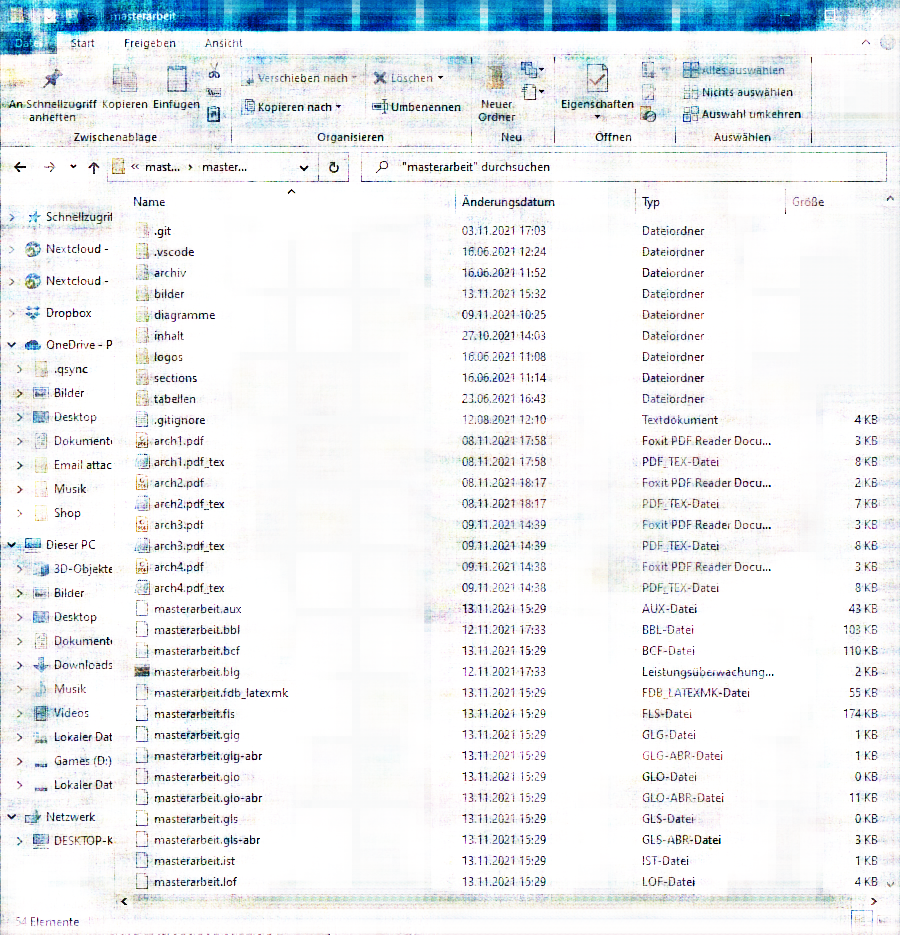
\includegraphics[width=\textwidth]{bilder/result_exp4/3_pred_a1.png}

  \caption{Experiment 4: Ausgabe des Autoencoders~\ref{a1} zu Bild 1 aus Abb.~\ref{exp4_image:1} in hoher Auflösung}
\end{figure}

\begin{figure} [ht]
  \centering
  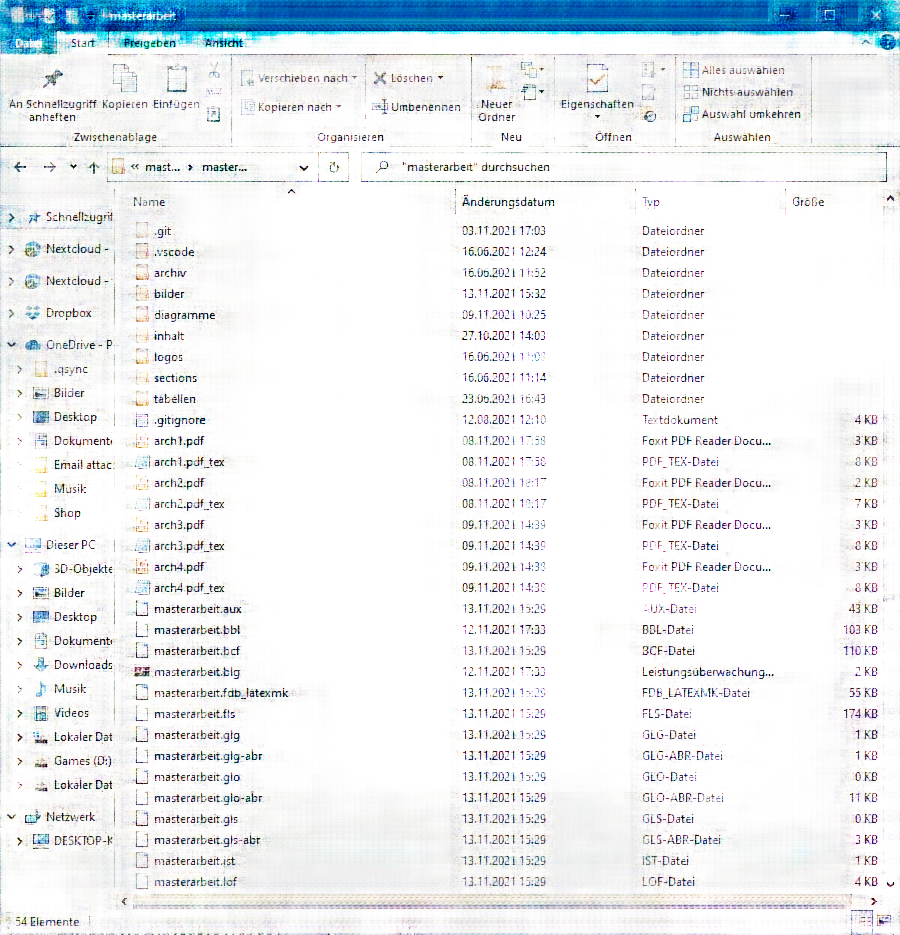
\includegraphics[width=\textwidth]{bilder/result_exp4/3_pred_a2.png}

  \caption{Experiment 4: Ausgabe des Autoencoders~\ref{a2} zu Bild 1 aus Abb.~\ref{exp4_image:1} in hoher Auflösung}
\end{figure}

\begin{figure} [ht]
  \centering
  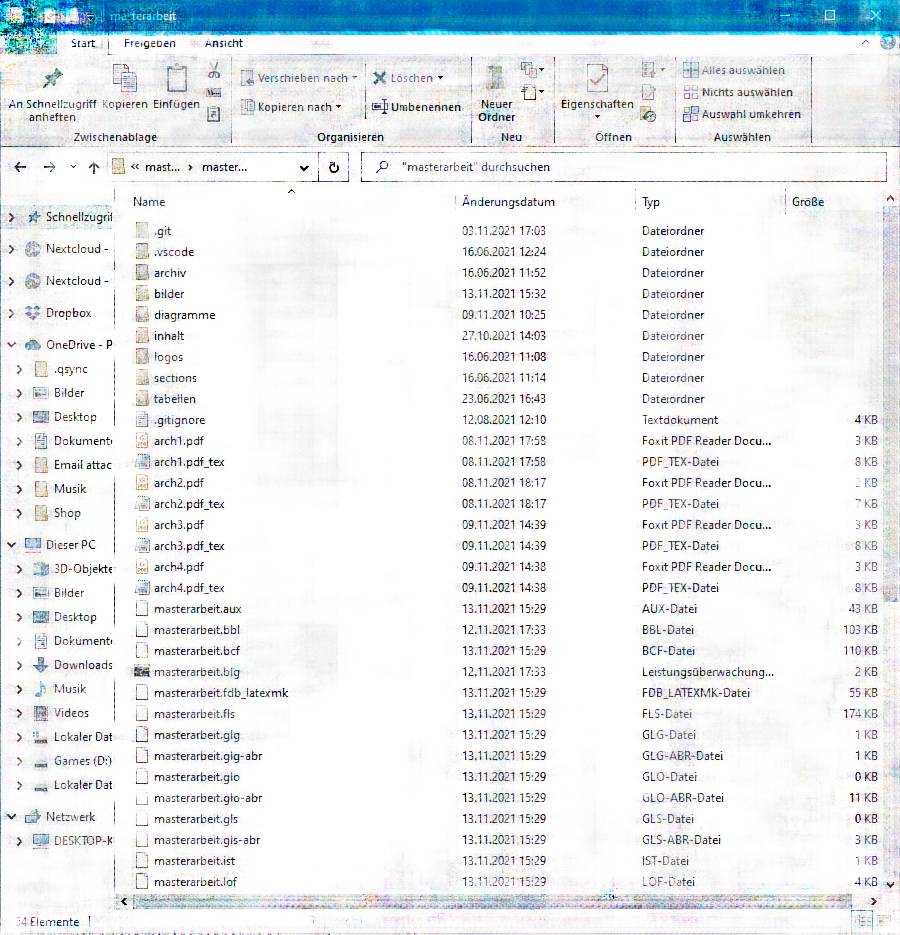
\includegraphics[width=\textwidth]{bilder/result_exp4/3_pred_a3.png}

  \caption{Experiment 4: Ausgabe des Autoencoders~\ref{a3} zu Bild 1 aus Abb.~\ref{exp4_image:1} in hoher Auflösung}
\end{figure}

\begin{figure} [ht]
  \centering
  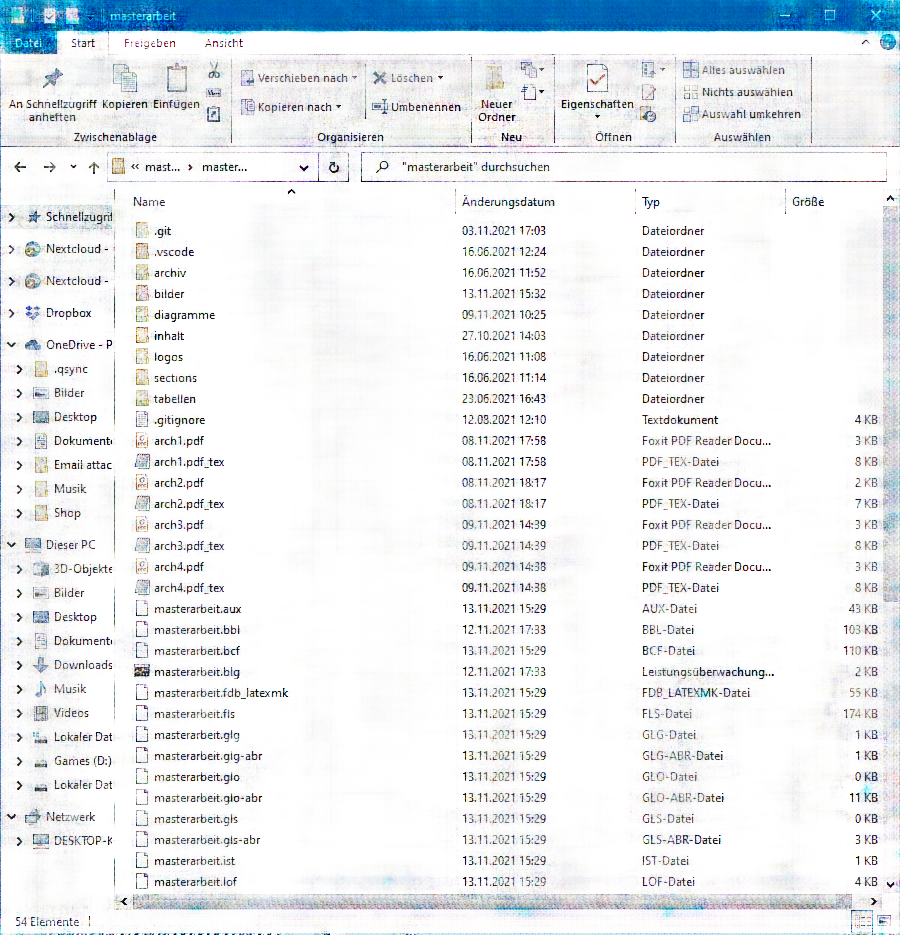
\includegraphics[width=\textwidth]{bilder/result_exp4/3_pred_a4.png}

  \caption{Experiment 4: Ausgabe des Autoencoders~\ref{a4} zu Bild 1 aus Abb.~\ref{exp4_image:1} in hoher Auflösung}
\end{figure}

\label{sec:appendix:exp4_2}
\begin{figure} [ht]
  \centering
  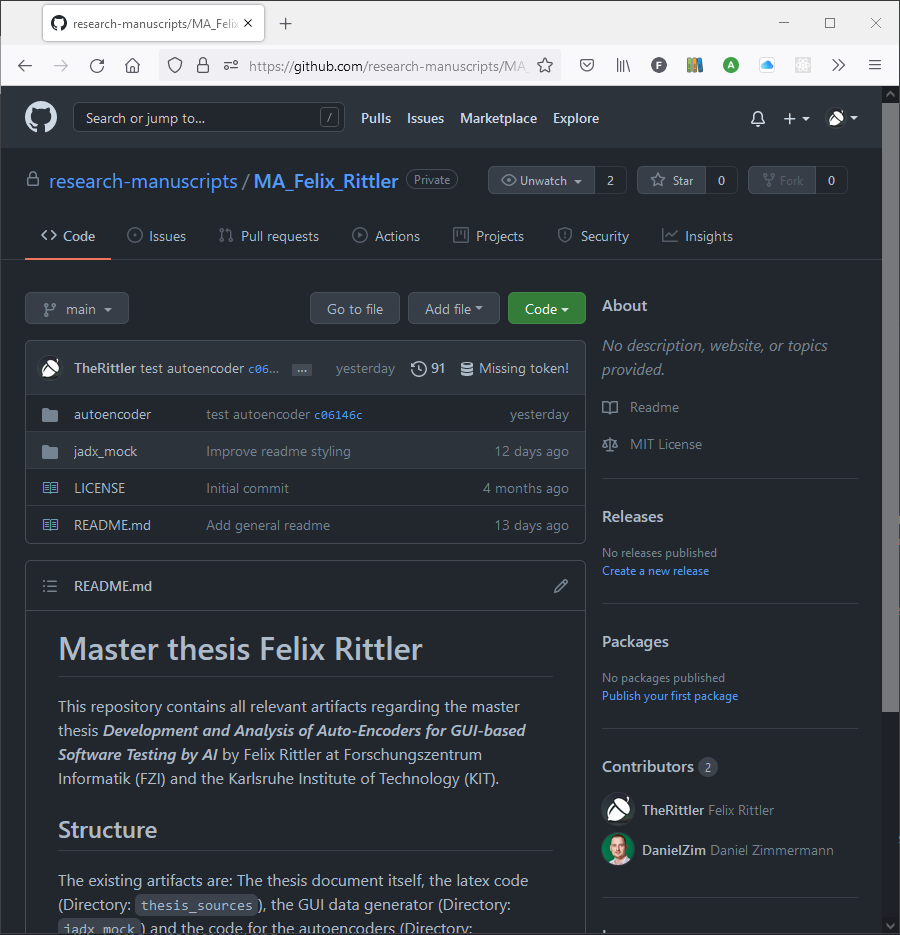
\includegraphics[width=\textwidth]{bilder/result_exp4/4.png}

  \caption{Experiment 4: Originalbild 2 aus Abb.~\ref{exp4_image:2} in hoher Auflösung}
\end{figure}

\begin{figure} [ht]
  \centering
  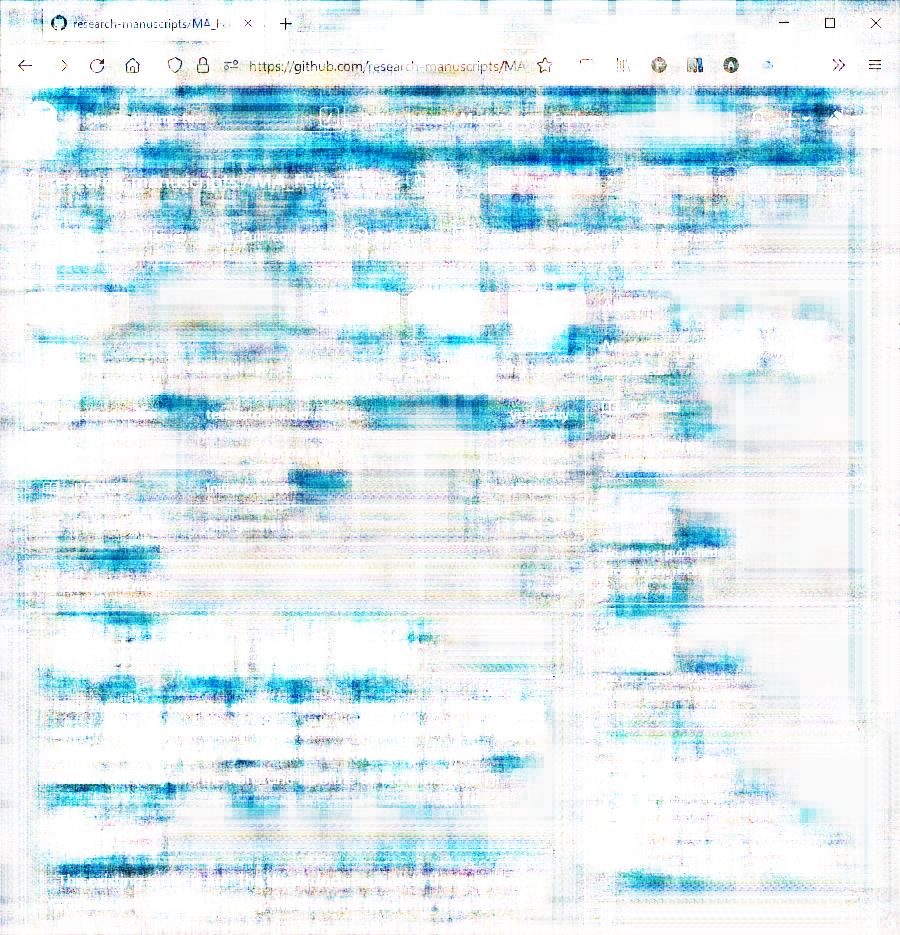
\includegraphics[width=\textwidth]{bilder/result_exp4/4_pred_a1.png}

  \caption{Experiment 4: Ausgabe des Autoencoders~\ref{a1} zu Bild 2 aus Abb.~\ref{exp4_image:2} in hoher Auflösung}
\end{figure}

\begin{figure} [ht]
  \centering
  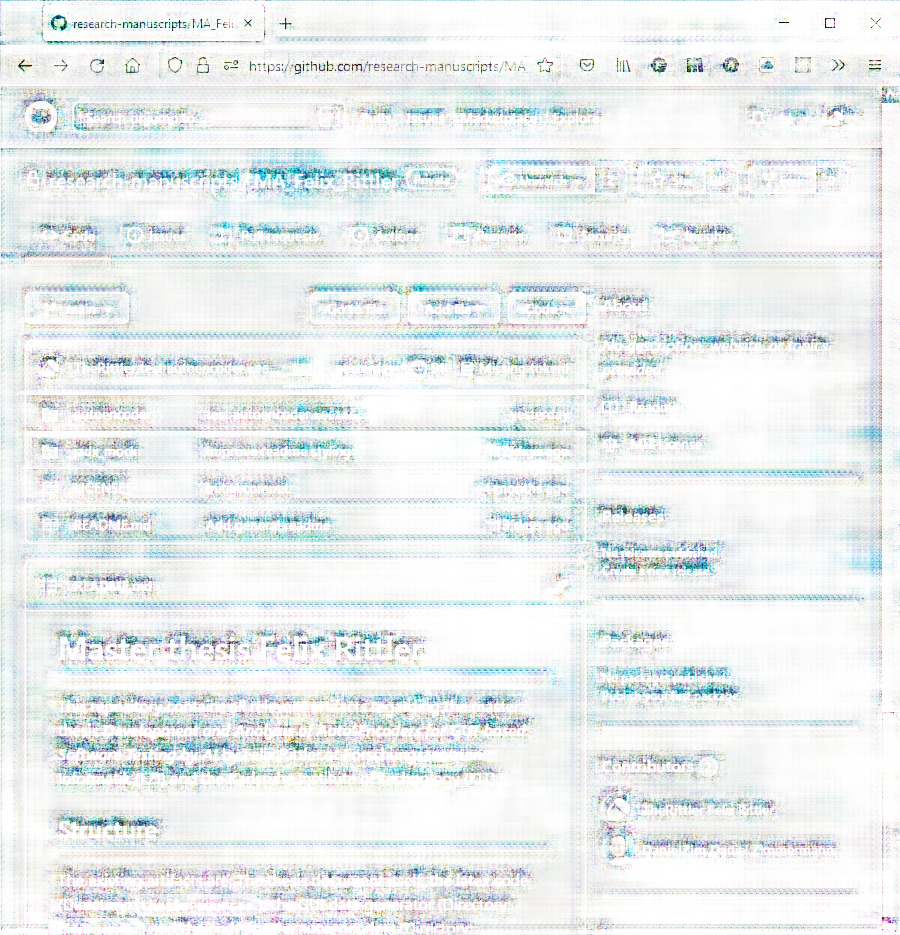
\includegraphics[width=\textwidth]{bilder/result_exp4/4_pred_a2.png}

  \caption{Experiment 4: Ausgabe des Autoencoders~\ref{a2} zu Bild 2 aus Abb.~\ref{exp4_image:2} in hoher Auflösung}
\end{figure}

\begin{figure} [ht]
  \centering
  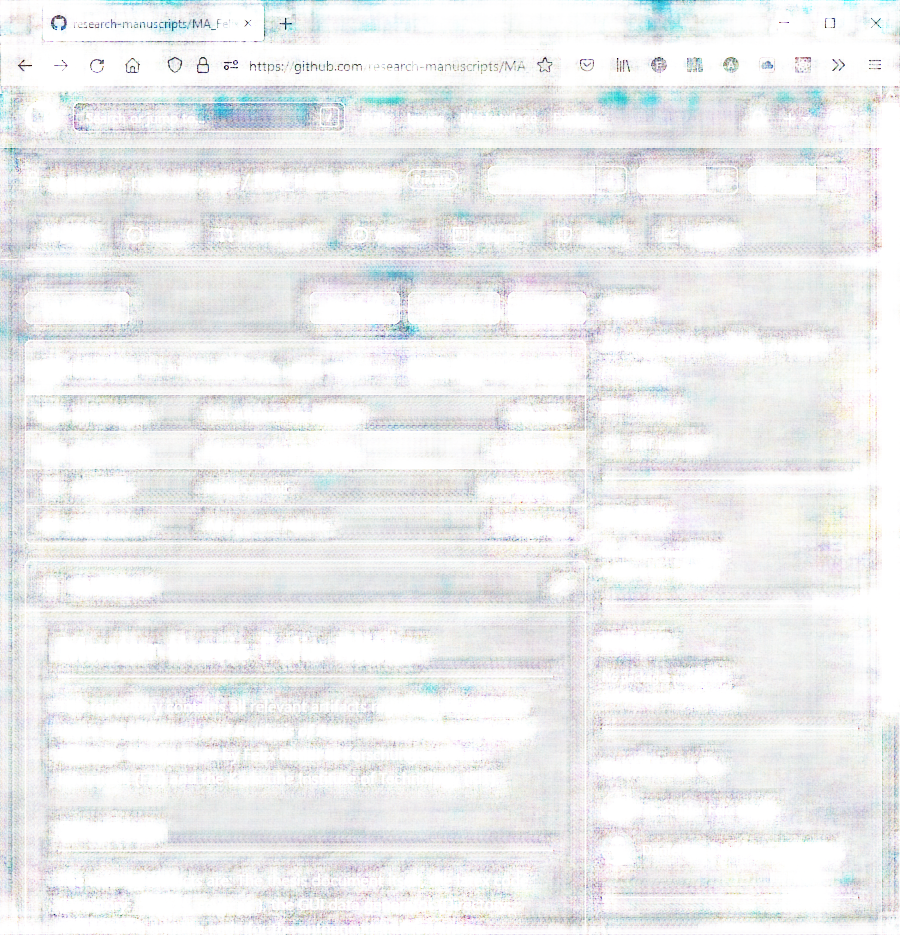
\includegraphics[width=\textwidth]{bilder/result_exp4/4_pred_a3.png}

  \caption{Experiment 4: Ausgabe des Autoencoders~\ref{a3} zu Bild 2 aus Abb.~\ref{exp4_image:2} in hoher Auflösung}
\end{figure}

\begin{figure} [ht]
  \centering
  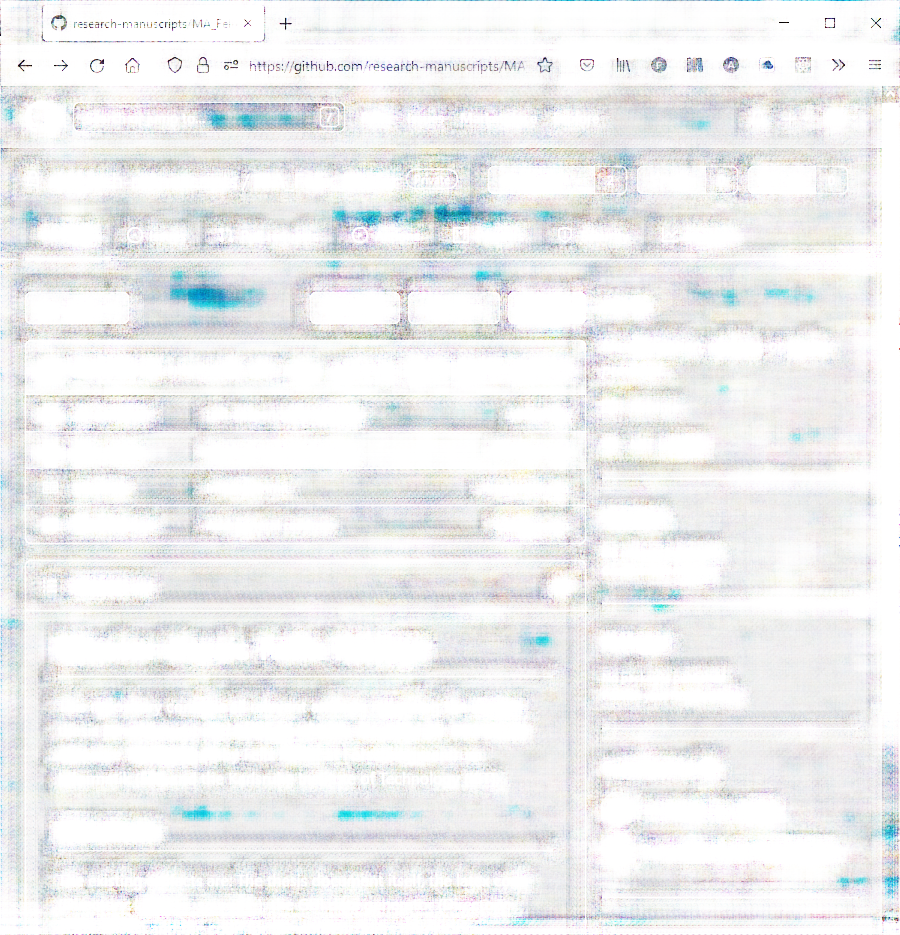
\includegraphics[width=\textwidth]{bilder/result_exp4/4_pred_a4.png}

  \caption{Experiment 4: Ausgabe des Autoencoders~\ref{a4} zu Bild 2 aus Abb.~\ref{exp4_image:2} in hoher Auflösung}
\end{figure}

\setcounter{figure}{0}

% \begin{figure} [ht]
%   \centering
%   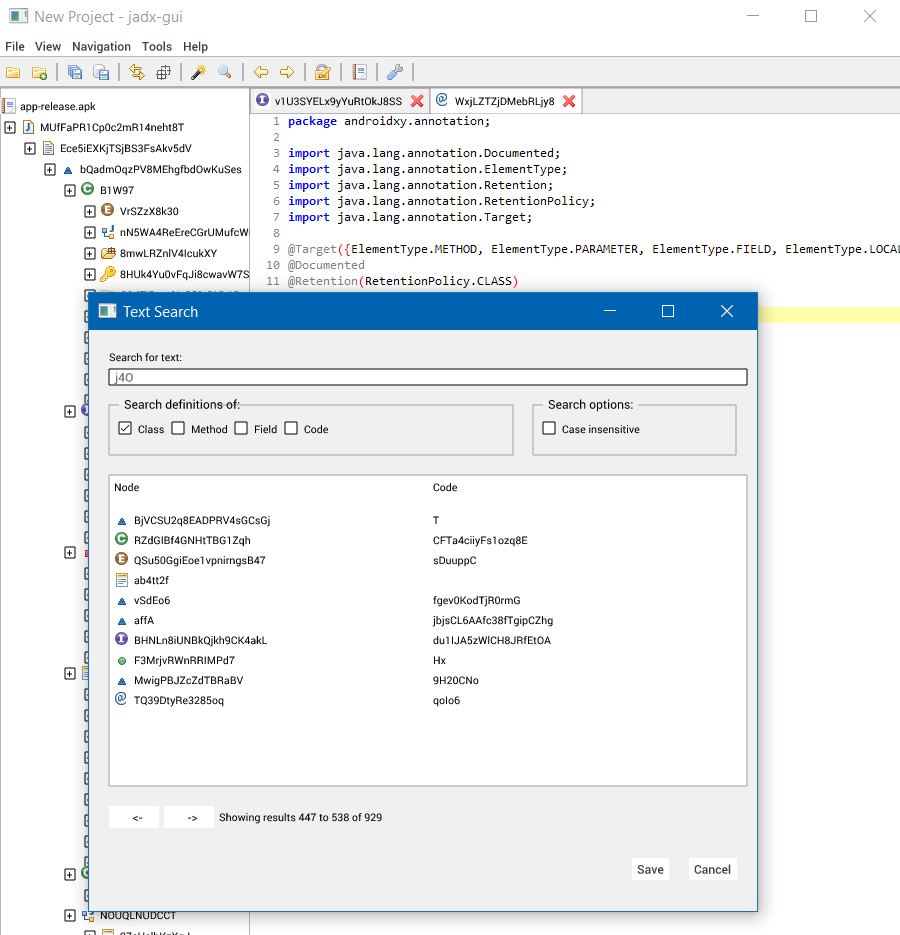
\includegraphics{bilder/result_exp2/0.png}
%   \caption{A figure}
% \end{figure}


%% ---------------------
%% | / Example content |
%% ---------------------